\documentclass[12pt,manuscript]{aastex}
\usepackage{savesym}
\savesymbol{tablenum}
\usepackage{siunitx}
\restoresymbol{SIX}{tablenum}
\usepackage{subcaption}
\usepackage{amsmath}
 
\begin{document}

\newcommand{\Msun}{M_\odot}
\newcommand{\Lsun}{L_\odot}
\newcommand{\Rsun}{R_\odot}
\newcommand{\Mearth}{M_\oplus}
\newcommand{\Learth}{L_\oplus}
\newcommand{\Rearth}{R_\oplus}
\newcommand{\Mjup}{M_{Jup}}
 
\title{On the Relation Between Intrinsic and RV-Traced Exoplanet Observations}
\author{Cail Daley}
\altaffiltext{1}{Department of Astronomy and Van Vleck Observatory,
Wesleyan University, Middletown, CT, 06459; {\tt
cdaley@wesleyan.edu}}


\begin{abstract}

The true exoplanet distribution across a given parameter (planet mass, semi-major axis, etc.)  is not, of course, perfectly traced by the distribution derived from radial velocity observations. 
This is due to many factors and biases, in particular the bias towards high-mass planets close to their host star. 
Assuming we understand these biases well, it should be possible to find the “true” exoplanet distribution that corresponds to the distribution traced by RV techniques. 
While such a goal falls outsides the scope of this project, I would like to take inspiration from this concept and explore the relations between intrinsic distributions and those traced by RV techniques.
This would involve creating synthetic radial velocity curves for hundreds/thousands of systems, varying the number of planets, planet masses and separations, etc. Then for each system, I will use some combination of nested sampling and MCMC methods to fit the data, allowing the distribution derived from RV data to be compared to the `true' data. 
I would like to emphasize that the goal of this project does not take the form of an attempt to directly learn about the intrinsic exoplanet distribution in our universe, but rather to learn about the relation between RV-observed and intrinsic distributions regardless of the form the distribution takes.

\end{abstract}


%give keywords (see subject headings in http://dopey.mcmaster.ca/AASTeX/)
\keywords{methods: statistical, numerical --- techniques: radial velocities --- 
planets and satellites: detection, fundamental parameters}
\newpage

\section{Introduction}
\label{section: intro}

The primary focus of exoplanetary science during its two decades of existence has been the identification and characterization of individual exoplanets.
This task is absolutely crucial to the field, as it generates a statistically significant sample of the exoplanet distribution that can in turn be used to constrain theories of planet formation, migration and so on.
NASA's exoplanet archive lists 3550 confirmed exoplanets; a large portion of these have been detected only in the past five years.
This sample has been built up with a wide variety of observational techniques, each sensitive to specific regions of the parameter space across which exoplanets are distributed. Some methods, like radial velocity or transit observations, are biased towards planets orbiting very close to their host star; others, like direct imaging, preferentially detect planets at large separations.

The presence of such biases invites the conclusion that the exoplanet distribution implied by the sample of observed exoplanets is not the same as the true or intrinsic distribution; the intrinsic distribution has been filtered through the biases specific to the various detection methods to produce the observed distribution. Indeed, we argue that for a given detection technique, we may think of the instrumental, observational, and statistical biases associated with that technique contributing to a mapping. This mapping transforms the intrinsic frequency distribution to an observed frequency distribution. It is dependent on a wide range of parameters (e.g. the planet eccentricity or the rotation rate of the host star) and may not have a functional form. Nevertheless, if the mapping for a given detection method can described (equivalent to the selection effects of the technique being well characterized), then it may be possible to recover information about the true exoplanet frequency distribution that is hidden in our observed distribution.

In the following pages, we apply this concept to the radial velocity detection technique. 
This involves: i) creating a synthetic `intrinsic' exoplanet distribution, ii) simulating a twenty-year radial velocity survey of the distribution, iii) fitting the observed lightcurves with Bayesian statistical methods, and iv) compiling the fit information to create an observed distribution. 
We emphasize that this work falls somewhere between a proof-of-concept and a reproduction of the biases inherent in the analytic equations discussed in Section \ref{section: survey} that govern radial velocity detectability.
Because the biases that affect the intrinsic-to-observed mapping are myriad, it is not within the scope of this project to characterize them all accurately. 
Instead we hope to take a (synthetic) data-based approach to illustrating the effect of these observations.
This leads us to state one of the guiding principles of this project:
\textit{eliminate or mitigate the effect of all biases other than those we are interested in characterizing}.
This principle will be used throughout this work to justify various assumptions.

In Section \ref{section: distribution} the  distribution is described, and simplifying assumptions are justified.
Section \ref{section: survey} discusses the survey, and
Section \ref{section: fitting} details the fitting process.
In Section \ref{section: results} we present the resulting observed exoplanet distribution, and compare it to the intrinsic distribution.
In Section \ref{section: conclusion} we summarize our results, relate our work to the current state of exoplanetology, and propose future work.
% The current state of the field is a product of countless hours of observations and analysis by both professional and amateur astronomers, and I would be remiss if I did not state my deep appreciation for their work.

% The true exoplanet distribution across a given parameter (planet mass, semi-major axis, etc.)  is not, of course, perfectly traced by the distribution derived from radial velocity observations. 
% This is due to a variety of factors and biases, e.g. the bias towards high-mass planets close to their host star. 
% Assuming we can accurately characterize these biases, it should be possible to find the “true” exoplanet distribution that corresponds to the distribution traced by RV techniques. 
% While such a goal falls outsides the scope of this project, I would like to take inspiration from this concept and explore the relations between intrinsic distributions and those traced by RV techniques. 
% This will be a primarily computational project, comprised of at least three major components: (i) creation of exoplanet distributions (ii) creation of an `observed' light curve for each planetary system in a distribution as part of a hypothetical RV survey, and (iii) fitting the lightcurve with MCMC (and possibly nested sampling) techniques. 
% Each component is discussed in a section below.
% As this project is still in its infancy in terms of implementation, I give a short description of my (planned) methodology and then mention some of the problems and questions I've been wrestling with in bullet points. I welcome all commentary, but the bullet points are the things I especially need help on.

\section{The Distribution}
\label{section: distribution}

The distribution is comprised of planetary systems; each system is defined by an inclination and a stellar mass. 
Each system is identical, with a inclination of \ang{90} and a stellar mass of \SI{1}{\Msun}.
Of course, fixing the inclination at any value is not realistic, and we hope to correct this in the future. 
Despite this we note that inclination is a purely observational parameter, unrelated to intrinsic exoplanet properties such as mass or semi-major axis, and so will not introduce systematic biases into the synthetic distribution.
Fixing the stellar mass has two justifications.
Stellar mass is correlated with a host of other properties (for example, luminosity or spectral line contrast) that bias the real-world observed exoplanet distribution in a variety of ways. 
As we are not able to account for these effects, fixing the stellar mass is the best way to prevent unknown biases into our sample. 
Second, the majority of exoplanet systems detected by radial velocity lie around solar-mass stars (as seen in Figure \ref{fig: solar mass}), so fixing the stellar mass at \SI{1}{\Msun} allows better comparison between synthetic and real-world distributions.

\begin{figure}[h]
  \centering
  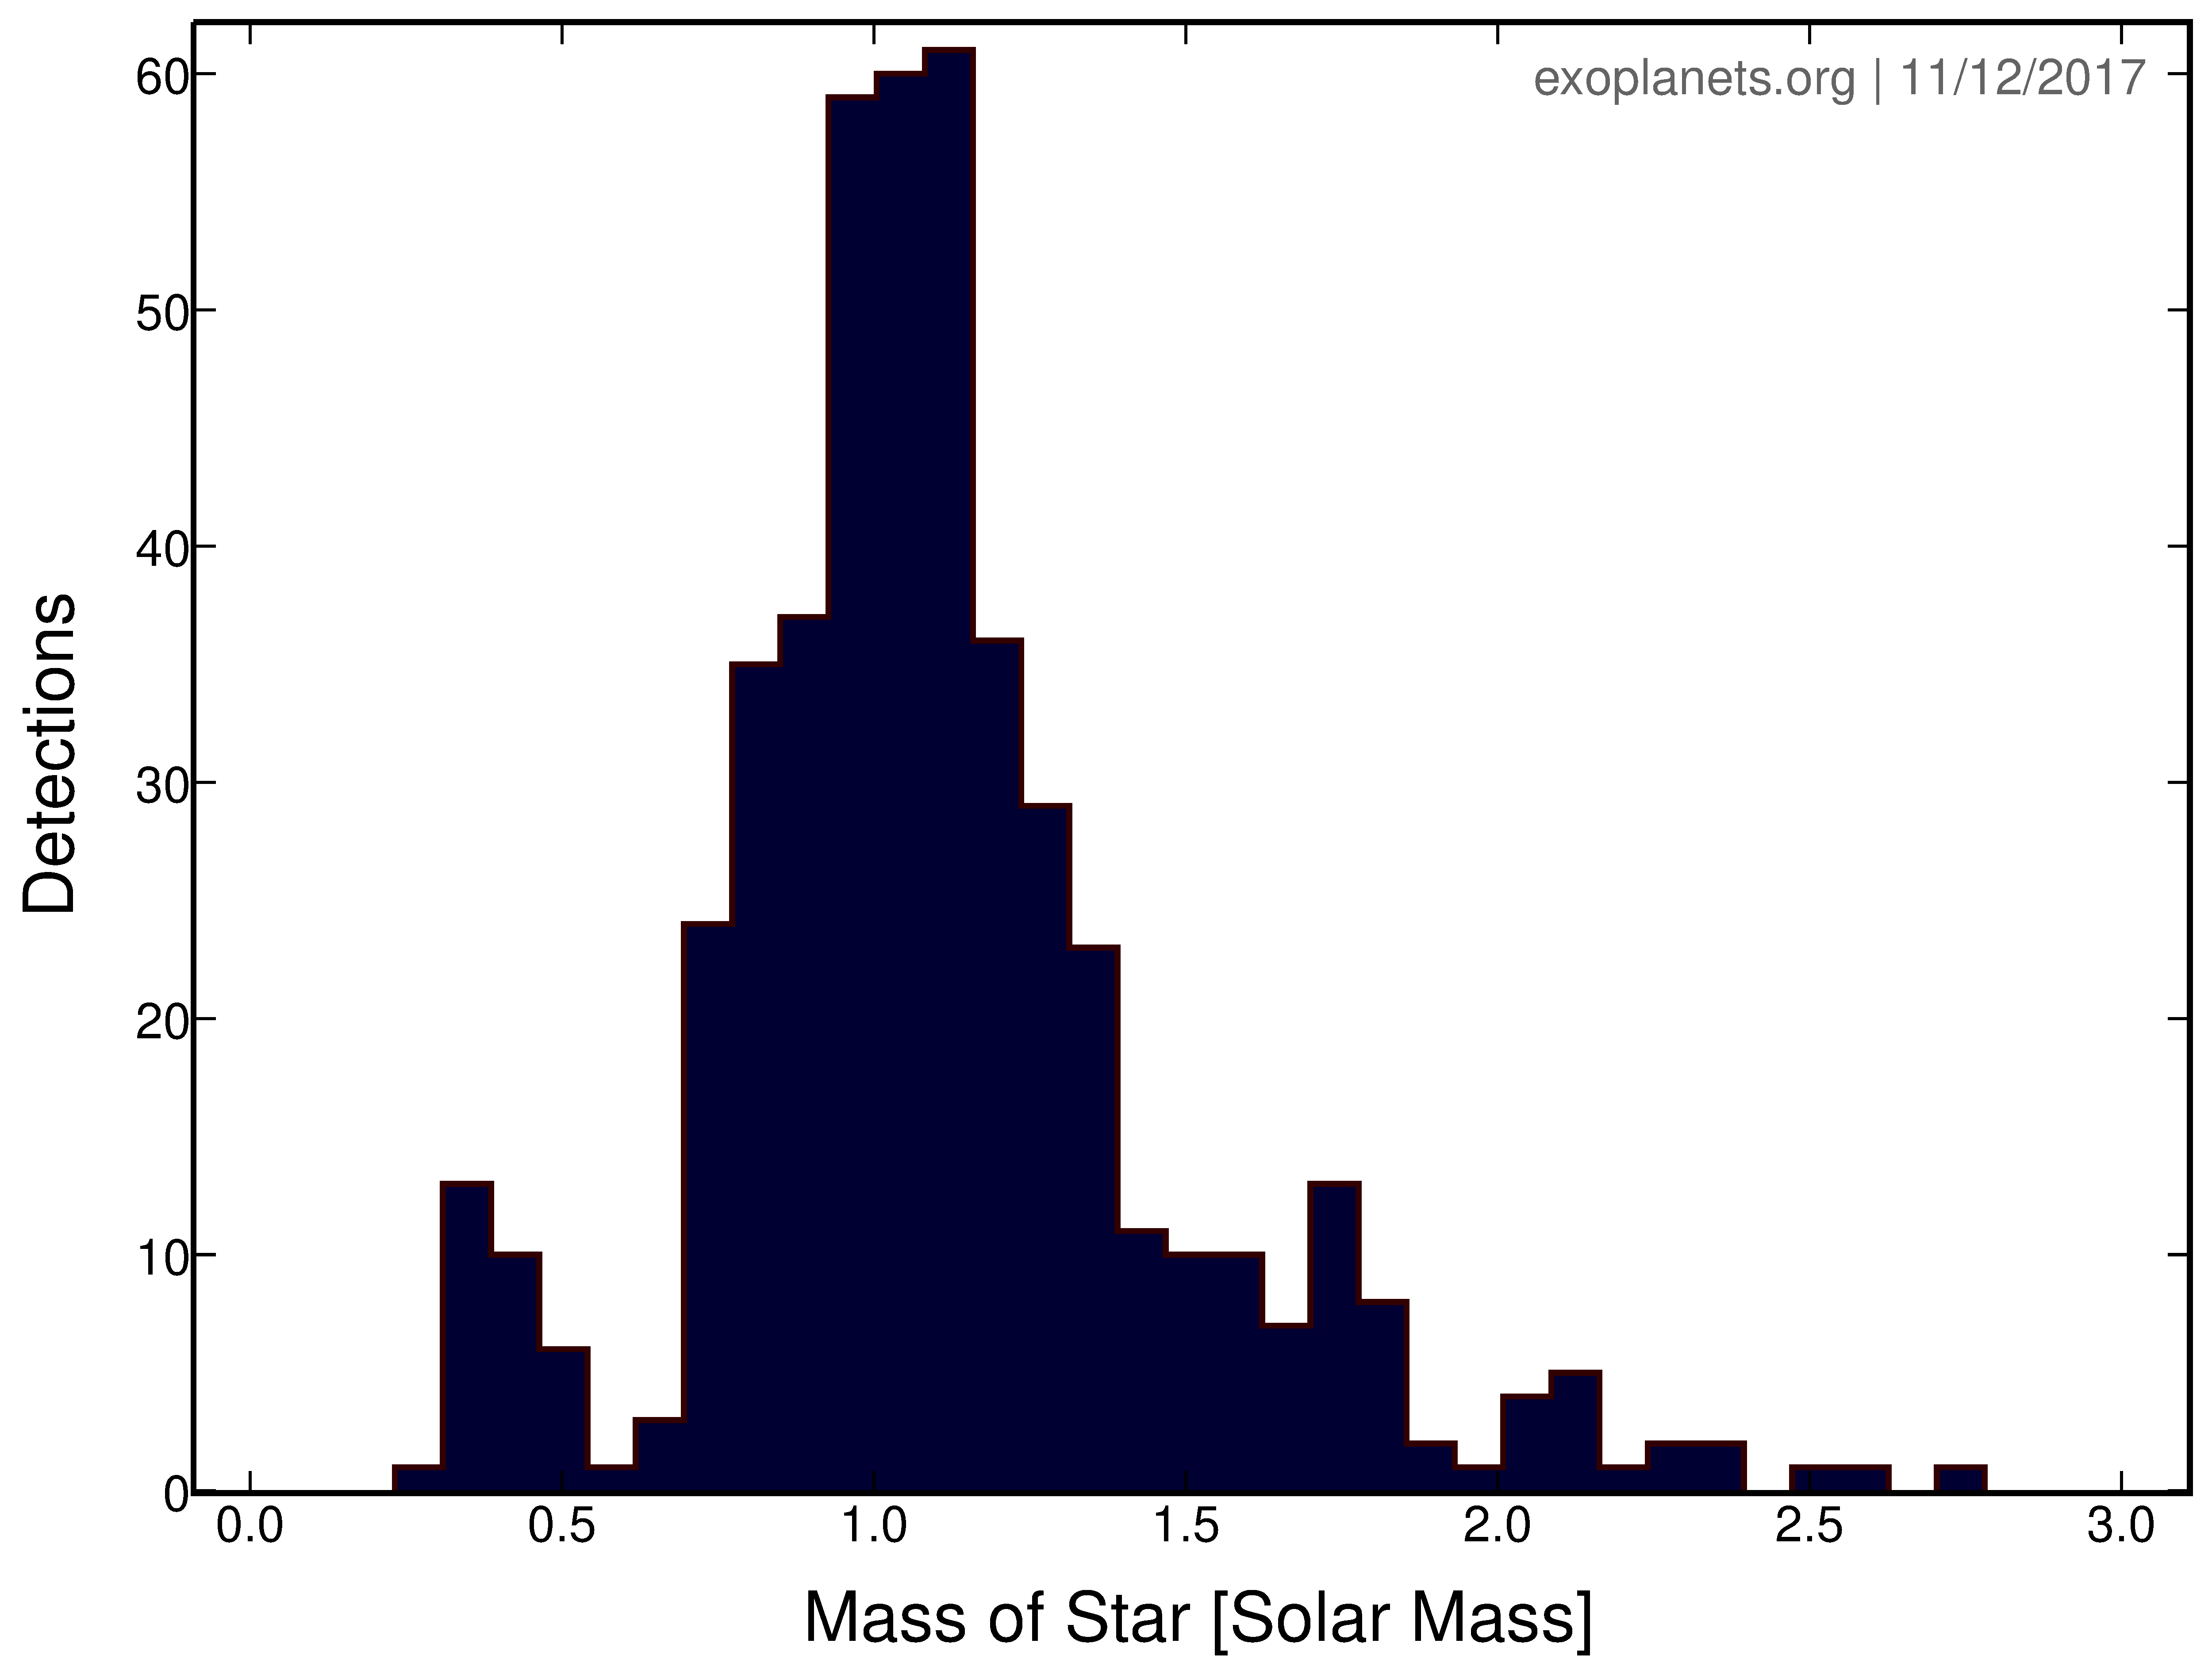
\includegraphics[width=0.5\linewidth]{../figures/solar_mass_detections}
  \caption{Number of exoplanet system detections as a function of stellar mass.}
  \label{fig: solar mass}
\end{figure}

Each system is assigned exactly one planet. 
Each planet is defined by a mass $m$, a semi-major axis $a$, an eccentricity $e$, an argument of periastron $\omega$, and time since periastron $t_0$. 
Eccentricity is set to zero for all planets; as $\omega$ is meaningless for $e=0$ it too is set to zero. 
The decision to fix eccentricity at zero was primarily motivated by difficulties in the fitting process (an expert in the field once once referred to eccentricity as a `bugaboo'). 
Exoplanet mass ranges between \SI{0.01}{\Mearth} and \SI{13}{\Mjup}, the brown dwarf mass limit. 
Semi-major axis ranges between \SI{0.1}{au}, below this fitting gets very inconsistent, and \SI{10}{au}. 
This upper limit corresponds to a period of $\sim \SI{30}{years}$, or 1.5 times the length of the survey discussed in the following section. 
As such, planets beyond \SI{10}{au} will have limited phase coverage, significantly limiting the confidence of detections.
Finally, $t_0$ is assigned a random number between 0 and the planet's period.\footnote{I actually made a mistake in the simulations presented in this draft---all the planets have $t_0=0$. It doesn't really matter anyways, since there's only one planet in each system.}
Planets are spaced logarithmically (in the final version..) between the boundaries given above, forming a two-dimensional logarithmic grid in $m-a$ parameter space (Figure \ref{fig: intrinsic_dist}). This allows easier comparison of the observed and intrinsic exoplanet distributions, as seen in Section \ref{section: results}.

\begin{figure}[h]
  \centering
  \includegraphics[width=0.5\linewidth]{../figures/intrinsic_dist}
  \caption{Intrinsic Exoplanet Distribution}
  \label{fig: intrinsic_dist}
\end{figure}


\section{Observations}
\label{section: survey}

Each exoplanet system is observed fifty times across the twenty year survey; the systemic radial velocity associated with a given date is calculated as follows. First, the mean anomaly $M$ is calculated from the planet's period $P$ and time since periastron passage $t_0$.
\begin{align}
  M = &2\pi \frac{(t-t_0)}{P} 
  \intertext{The eccentric anomaly $E$ can be determined from $M$ by solving Kepler's Equation with a numerical solver:}
  M = &E - e \sin E 
  \intertext{and the true anomaly $f$ can be determined from $E$ as follows:}
  f = &2\arctan \left( \sqrt{\frac{1 + e}{1 - e}} \frac{\sin E}{\cos E} \right)
  \intertext{Finally, the radial velocity of the star $v_{r,1}$ can be calculated now that $f$ is known.}
  v_{r,1} = &\sqrt{ \frac{G}{(m_1 + m_2)a(1-e^2)}} m_2 \sin i \\
  &\cdot (\cos(\omega + f) + e \cos \omega)
\end{align}
This process is repeated for each date in the time series, generating a synthetic light curve.
The resulting resulting curves agree well with theoretical predictions; for a $e=0$ Jupiter analogue around a solar analogue, We derive a $K_1$ of \SI{28.42}{m/s}, compared to the theoretical value of \SI{28.43}{m/s}.  
To make observations more realistic, Gaussian \SI{1}{m/s} noise is applied to produce the `observed' radial velocity curve.  We ignore all stellar noise contributions due to the difficulty in accurately characterizing them, and because of correlations between stellar noise and exoplanet characteristics (by way of spectral type, for example).

\begin{figure}
  
  \begin{subfigure}[b]{.9\linewidth}
  \includegraphics[width=\linewidth]{../figures/sample_curve}
  \end{subfigure}
  
  \begin{subfigure}[b]{.9\linewidth}
  \includegraphics[width=\linewidth]{../figures/sample_curve_noisy}
  \end{subfigure}
  
  \caption{Top: Radial velocity curve of a four-planet system around a solar analogue, with planet parameters listed at the top of the figure. The star is a solar analogue. Bottom: The same system, but with \SI{1}{m/s} Gaussian noise added.}
  \label{fig: lightcurve}
\end{figure}


To produce self-consistent data that reasonably approximate real-world radial velocity observations, we assume that all of the synthetic observations are taken as part of the same radial velocity survey.
The survey is conducted over twenty years, with twenty observations taken each night.
Imposing the requirement that each system is observed fifty times yields a exoplanet system size of $\sim 3000$ exoplanets. 
Observations are spaced logarithmically between \SI{1e5}{days} and $\num{1e5} + (20 \times \SI{365.25}{days})$ and then shifted back by \SI{1e5}{days}, so that the first observation occurs at $t=0$.
Because logarithmic spacing converges to linear spacing for very large numbers, this method results in almost---but not quite---linearly spaced observations.
In fact, the observations are spaced in such a way that breadth of relevant frequency space is well sampled. 
Figure \ref{fig: periods} shows both the intrinsic and observed lightcurves of two planets---one short-period and one long-period ---as observed by the survey.
In both cases, coverage of the entirety of phase space is recovered.

\begin{figure}
  \centering
  
  \begin{subfigure}[b]{.45\linewidth}
  \includegraphics[width=\linewidth]{../figures/long_P_no_fold}
  \end{subfigure}
  \begin{subfigure}[b]{.45\linewidth}
  \includegraphics[width=\linewidth]{../figures/short_P_no_fold}
  \end{subfigure}
  
  
  \begin{subfigure}[b]{.45\linewidth}
  \includegraphics[width=\linewidth]{../figures/long_P_folded}
  \end{subfigure}
  \begin{subfigure}[b]{.45\linewidth}
  \includegraphics[width=\linewidth]{../figures/short_P_folded}
  \end{subfigure}

  \caption{The effect of logarithmic-almost-linear spacings between observations. On the left, the time series lightcurve (above) and phase-folded lightcurve (below) for a long-period ($\sim \SI{7000}{day}$) exoplanet. On the right, the same two plots for a short-period ($\sim \SI{0.1}{day}$) exoplanet. At both extremes, the entirety of phase space is well sampled.}
  \label{fig: periods}
\end{figure}



\section{Fitting the Data}
\label{section: fitting}

With twenty years of observational data in hand, analysis can be performed. 
To recover exoplanet properties like mass or semi-major axis we use the nested sampling fitting code \texttt{PyMultiNest} \citep{buchner14}.
\texttt{PyMultiNest} is a Python implementation of the Bayesian inference algorithm \texttt{MULTINEST} \citep{feroz09}.
While an in-depth discussion of the algorithm is outside the scope of this paper, we note that it directly calculates the evidence by transforming a $n$-dimensional integral over all of parameter space (i.e. the prior volume) to a 1-dimensional sum across all likelihood values. 
This allows direct comparison between models with different parameter spaces.
The reader is encouraged to refer to the original \texttt{MULTINEST} paper if they find themselves to be curious.

The creation of model radial velocity curves exactly follows the procedure described in Section \ref{section: survey}.
Tens to hundreds of thousands of model curves with varying values of $m, a$ and $t_0$ ($e$ and $\omega$ are fixed to zero) are created for each system, and the log likelihood $L=-\chi^2/2$ is used to asses the quality of each model.
This effectively maps out parameters space so that the maximum likelihood (or best fit) parameters may be estimated.
Mass and semi-major axis are sampled logarithmically with uniform priors such that $-2.5 < \log m < \log (\SI{13}{\Mjup}) + 0.2$ and $-2.5 < \log a < 1.5$. 
Logarithmic sampling was chosen to better cover the four and three orders of magnitude traversed by $m$ and $a$, respectively.

Exoplanet detection is determined after the data has been fit. 
If the best-fit model peak signal-to-noise (SNR) ratio is greater than one, an exoplanet with said best-fit parameters is `detected.'
% In 14 planet sample with true SNR < 0.5, fit SNR was always less than 1.

% Once all the systems in a distribution have been fit, we can compare the `true' exoplanet distribution to the distribution constructed from the best fit model parameters from each system. While it will be difficult to make statements about our particular exoplanet distribution, it should be possible to make general statements about the regions of exoplanet parameter space that RV observations are sensitive to.
% 
% \begin{enumerate}
%   \item Once I have the two distributions, what other cool analyses could I do?
% \end{enumerate}

\section{Results}
\label{section: results}

\begin{figure}[h]
  \centering
  
  \begin{subfigure}[b]{.45\linewidth}
  \includegraphics[width=\linewidth]{../figures/planets2_intrinsic}
  \end{subfigure}
  \begin{subfigure}[b]{.45\linewidth}
  \includegraphics[width=\linewidth]{../figures/planets2_observed}
  \end{subfigure}
  \caption{A comparison of the intrinsic (left) and observed (right) distributions, color-coded by the best-fit model SNR. Planets with SNR $< 1$ are counted as nondetections.}
  \label{}
\end{figure}

\begin{figure}[h]
  \centering
  \includegraphics[width=0.9\linewidth]{planets2_comparison}
  \caption{A corner-type plot showing the correlations between the intrinsic mass distribution, the intrinsic semi-major axis distribution, the fit mass distribution, and the fit semi-major axis distribution. Again, the each planet is color-coded by the best-ft model SNR. Planets with SNR $< 1$ are counted as nondetections.}
  \label{}
\end{figure}

\begin{figure}[h]
  \centering
  \includegraphics[width=0.9\linewidth]{planets2_comparison_dropped}
  \caption{A corner-type plot showing the correlations between the intrinsic mass distribution, the intrinsic semi-major axis distribution, the fit mass distribution, and the fit semi-major axis distribution. Again, the each planet is color-coded by the best-ft model SNR. Planets with SNR $< 1$ are counted as nondetections, and have been dropped. As such this plot shows the preliminary comparison between intrinsic and detected observations.}
  \label{}
\end{figure}

\section{Conclusion}
\label{section: conclusion}

\begin{thebibliography}{}

\bibitem[Buchner et al.(2014)]{buchner14} Buchner, J., Georgakakis, A., Nandra, K., et al.\ 2014, \aap, 564, A125

\bibitem[Dumusque et al.(2017)]{dumusque17} Dumusque, X., Borsa, F., Damasso, M., et al.\ 2017, \aap, 598, A133 

\bibitem[Feroz et al.(2009)]{feroz09} Feroz, F., Hobson, M.~P., \& Bridges, M.\ 2009, \mnras, 398, 1601 

\bibitem[Traub(2016)]{traub16} Traub, W.~A.\ 2016, arXiv:1605.02255 

\bibitem[Winn \& Fabrycky(2015)]{winn&fabrycky15} Winn, J.~N., \& Fabrycky, D.~C.\ 2015, \araa, 53, 409 

\end{thebibliography}

 \end{document}
